\documentclass[hyperref=colorlinks]{beamer}
\mode<presentation>
\usetheme{iclpt}
\setbeamertemplate{navigation symbols}{}
\setbeamertemplate{headline}{
  \begin{beamercolorbox}[leftskip=.2cm,rightskip=.2cm,topskip=.2cm,ht=1.1cm,dp=0.1cm,wd=\textwidth]{institute in head/foot}
    
\includegraphics[height=1cm]{icl.pdf}
    \hfill
    
\includegraphics[height=1cm]{../Pics/CMS-Color.pdf}
  \end{beamercolorbox}
}
\setbeamertemplate{footline}{
  \begin{beamercolorbox}[ht=.35cm,dp=0.2cm,wd=\textwidth,leftskip=.3cm]{author in head/foot}%
    \begin{minipage}[c]{5cm}%
      \usebeamerfont{author in head/foot}
      \insertshortauthor 
      \insertshorttitle
    \end{minipage}\hfill%
    \hfill
    \insertframenumber{} / \ref{lastframe}
    %\hfill
    \begin{minipage}{6cm}
      \hfill
      %\insertshorttitle
    \end{minipage}
  \end{beamercolorbox}%
}

\definecolor{beamer@icdarkblue}{RGB}{0,51,102}
\definecolor{beamer@icmiddleblue}{RGB}{0,82,150} 
\definecolor{beamer@iclightblue}{RGB}{200,212,232}
\definecolor{beamer@icmiddlered}{RGB}{204,51,0}
\definecolor{beamer@iclightred}{RGB}{232,212,32}

\usepackage{tikz}
\usetikzlibrary{arrows,shapes,backgrounds}
\usepackage{color}
\usepackage{tabularx,colortbl}
\usepackage{graphicx}
\usepackage{pdfpages}
\usepackage{feynmp}
\usepackage{rotating}
\usepackage{moresize}
\usepackage{slashed}
\usepackage{xcolor,colortbl}
\DeclareGraphicsRule{*}{mps}{*}{}
\hypersetup{colorlinks=false}

\title[Invisible Higgs at CMS]{\vspace{-0.2cm} Searches for invisible decays of the Higgs boson with the CMS detector}
\author[P. Dunne]{\underline{P. Dunne} - Imperial College London} % A.M. Magnan and A. Nikitenko Joao Pela with \\ R. Aggleton, J. Brooke: Bristol \\ C.Asawangtrakuldee, Q.Li: Peking \\ P. Srimanobhas: Chulalongkorn \\ S. Kumar, K. Mazumdar: Mumbai}
\titlegraphic{
  \vspace{-0.4cm}
%  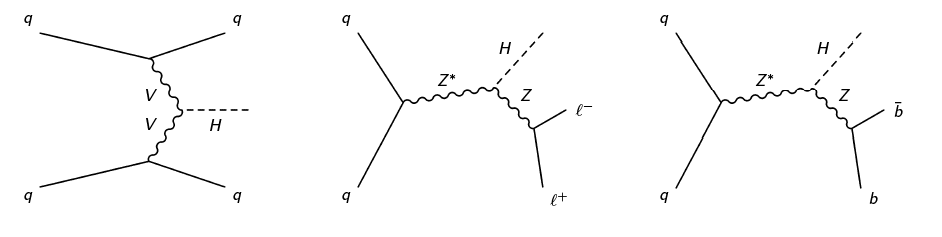
\includegraphics[width=\textwidth]{TalkPics/invcomb021213/feyndiags}
  \begin{fmfgraph*}(100,70)
          \fmfleft{i1,i2}
          \fmfright{o1,o2,o3}
          \fmf{fermion}{i1,v1,o1}
          \fmf{fermion}{i2,v2,o3}
          \fmf{phantom,tension=4/5}{v1,v2}
          \fmffreeze
          \fmf{photon,label=$W,,Z$}{v1,v3}
          \fmf{photon,label=$W,,Z$}{v2,v3}
          \fmf{dashes}{v3,o2}
          \fmflabel{$q$}{i1}
          \fmflabel{$q$}{i2}
          \fmflabel{$q$}{o1}
          \fmflabel{$q$}{o3}
          \fmflabel{$H$}{o2}

        \end{fmfgraph*}
}
\date{}
\begin{document}
\tikzstyle{every picture}+=[remember picture]
\tikzstyle{na} = [baseline=-.5ex]
\begin{fmffile}{pgrfeyndiags}

  %TITLE PAGE
  \section{Title}
  \begin{frame}
    \titlepage
    
  \end{frame}

  \begin{frame}
    \frametitle{Introduction}
    \begin{itemize}
    \item CMS and the LHC
    \item Why look for invisbly decaying Higgs bosons?
    \item How do you look for something invisible?
    \item What do we see?
    \end{itemize}
  \end{frame}

  %!!MORE DETAIL ON LHC AND CMS
  \begin{frame}
    \frametitle{CMS and the LHC}
    \begin{center}
      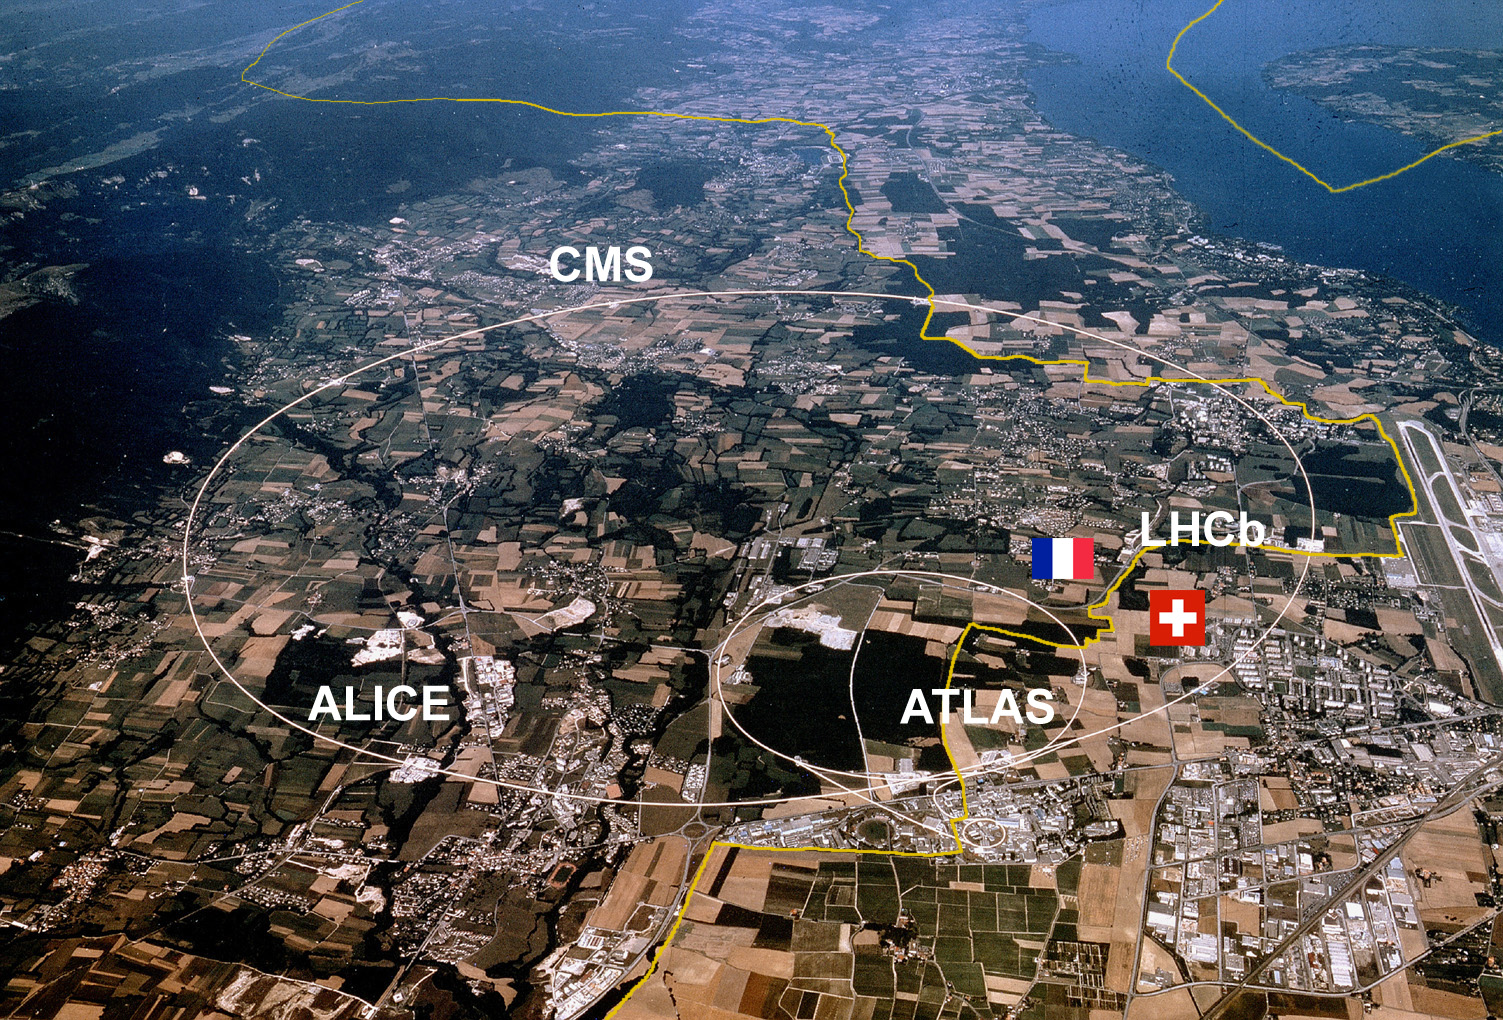
\includegraphics[width=.9\textwidth]{TalkPics/cern-lhc-aerial.jpg}
    \end{center}
  \end{frame}
  
  \begin{frame}
    \frametitle{CMS}
    \centering
    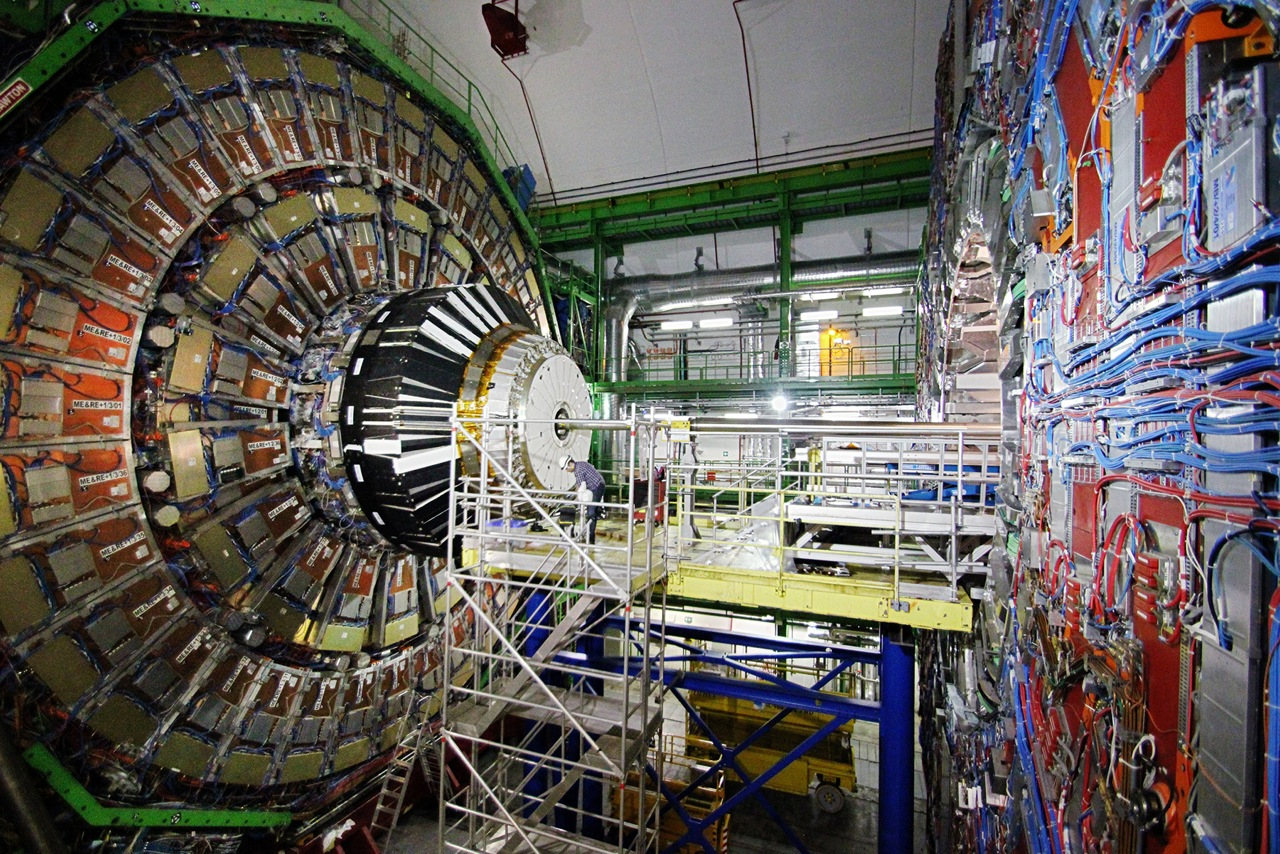
\includegraphics[height=.85\textheight]{TalkPics/sgs120315/cmsphoto.jpeg}
  \end{frame}

  \begin{frame}
    \frametitle{CMS}
    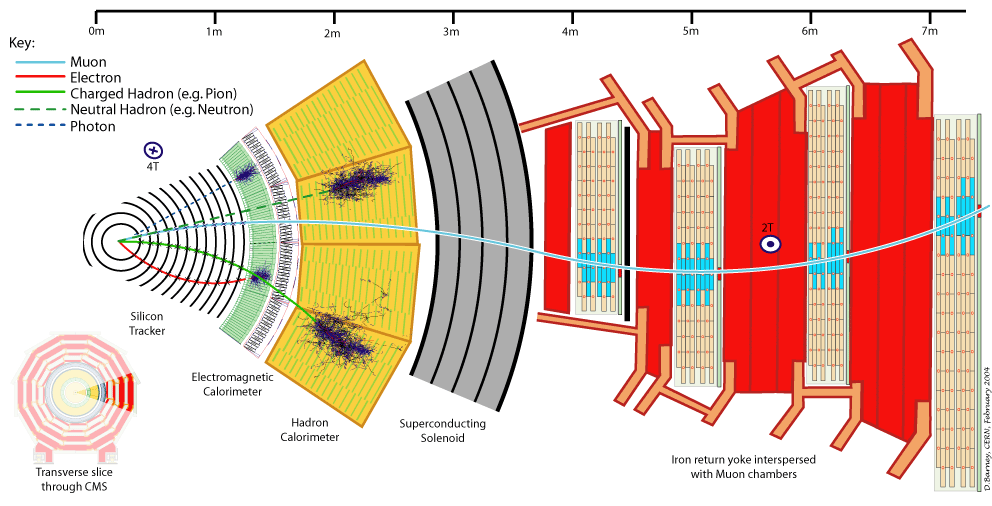
\includegraphics[width=\textwidth]{TalkPics/CMS_Slice.png}
  \end{frame}

  \begin{frame}
    \frametitle{The Higgs boson}
    \begin{columns}
      \column{.5\textwidth}
      \begin{itemize}
      \item Explains mass in the Standard model (SM)
        \begin{itemize}
          \color{beamer@icmiddleblue}
        \item Every particle with mass interacts with the Higgs
        \end{itemize}
      \item SM compatible Higgs boson observed at the LHC
        \begin{itemize}
          \color{beamer@icmiddleblue}
        \item SM compatible doesn't mean incompatible with other theories
        \end{itemize}
      \end{itemize}
      \column{.5\textwidth}
      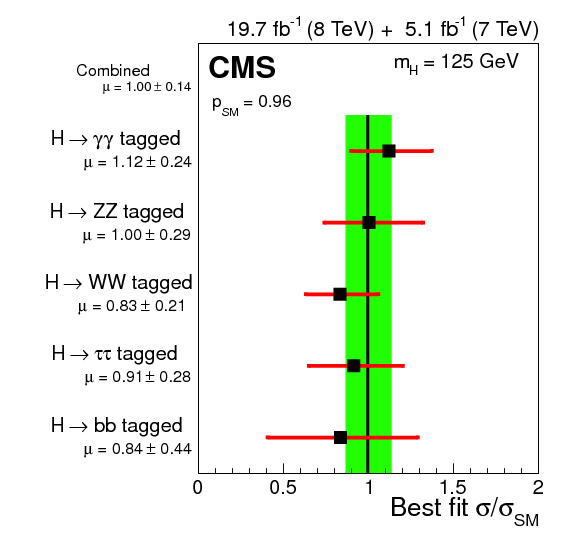
\includegraphics[width=\textwidth]{TalkPics/IOP2015/decaylimits.png}
    \end{columns}
  \end{frame}

  \begin{frame}
    \frametitle{Dark matter}
    \begin{itemize}
      \item What do we know?
        \begin{itemize}
          \color{beamer@icmiddleblue}
        \item Cold, massive, weakly interacting
        \end{itemize}
      \item All other massive particles get mass from Higgs coupling
      \item If dark matter is light enough the Higgs will decay to it
      \item Look for invisibly decaying Higgs..
    \end{itemize}
    \centering
     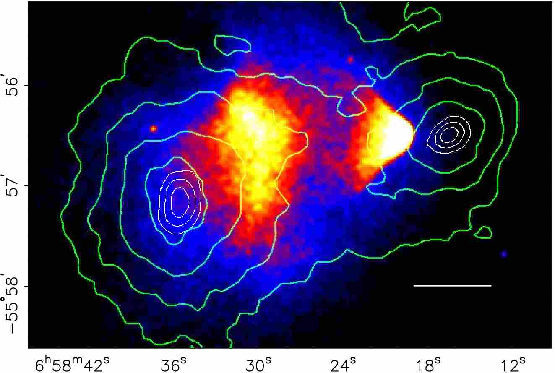
\includegraphics[clip=true,trim=0 0 0 0,height=.5\textheight,width=.5\textwidth]{TalkPics/sgs120315/bulletcluster.png}
       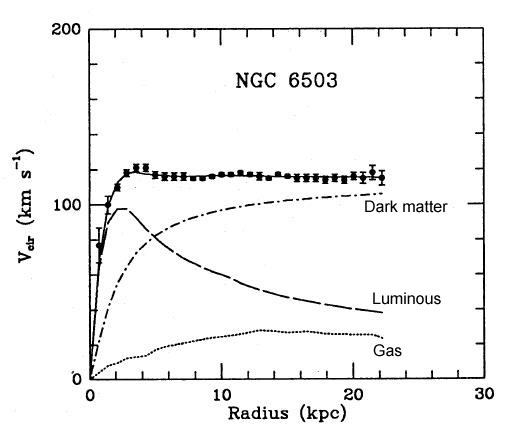
\includegraphics[clip=true,trim=0 0 0 0,height=.53\textheight,width=.5\textwidth]{TalkPics/sgs120315/rotationcurve.jpg}
       %!!PROBLEMS WITH THE SM
       %!!MUST STUDY WHAT WE KNOW IN DETAIL TO LOOK FOR DEVIATIONS AND LOOK FOR NEW PARTICLES


   \end{frame}

  \begin{frame}
    \frametitle{How do you look for something invisible:\\ Associated production}
    \begin{itemize}
    \item Higgs not always created alone
    \item Look for momentum imbalance
    \end{itemize}
    \centering
    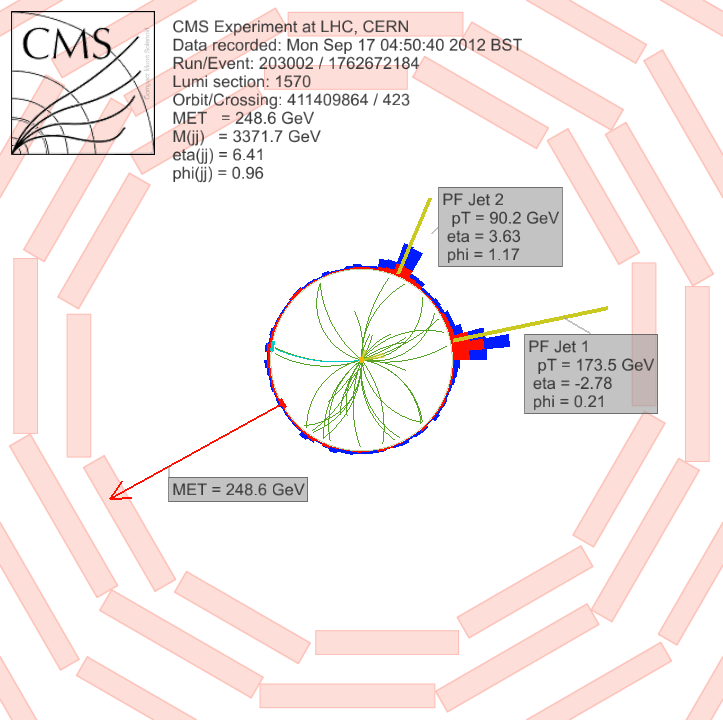
\includegraphics[width=.5\textwidth]{TalkPics/sgs120315/vbfevent.png}
  \end{frame}        

   \begin{frame}
     \frametitle{How do you look for something invisible:\\ VBF}
     
     \begin{itemize}
     \item Three main types of Higgs associated production:
       \begin{itemize}
         
       \item[] \tikz[na] \node (ggH) {ggH: high rate, normally no visible products};        
       \item[] \tikz[na] \node (VBF) {VBF: medium rate, jets+MET final state};        
       \item[] \tikz[na] \node (ZH) {ZH: low rate, leptons/b jets+MET final state};        
       \end{itemize}
     \end{itemize}


     \begin{columns}
       \column{.5\textwidth}
           \begin{tikzpicture}%[show background grid]
            \node [inner sep=0pt,above right]
            {\includegraphics[height=.45\textheight,width=.9\textwidth]{../../Reports/Firstyearreport/Higgs_XS_8TeV_lx.pdf}};
 %           \fill (0,0) circle (2pt);

            \path (1.2,3.1) coordinate (ggHl)
                  (1.9,2.2) coordinate (VBFl)
                  (2.6,1.2) coordinate (ZHl);
          \end{tikzpicture}
       \column{.5\textwidth}
       \begin{tikzpicture}
         \node[inner sep=0pt,above right]
              {\begin{fmfgraph*}(80,70)
                  \fmfleft{i1,i2}
                  \fmfright{o1,o2,o3}
                  \fmf{fermion}{i1,v1,o1}
                  \fmf{fermion}{i2,v2,o3}
                  \fmf{phantom,tension=4/5}{v1,v2}
                  \fmffreeze
                  \fmf{photon,label=$W,,Z$}{v1,v3}
                  \fmf{photon,label=$W,,Z$}{v2,v3}
                  \fmf{dashes}{v3,o2}
                  \fmflabel{$q$}{i1}
                  \fmflabel{$q$}{i2}
                  \fmflabel{$q$}{o1}
                  \fmflabel{$q$}{o3}
                  \fmflabel{$H$}{o2}
              \end{fmfgraph*}};
              \path (2.9,3.1) coordinate (VBFdiag);

       \end{tikzpicture}
     \end{columns}

    \begin{tikzpicture}[overlay]
      \path[->,blue,thick] (ggH.west) edge [bend right] (ggHl);
      \path[->,red,thick] (VBF.west) edge [bend right] (VBFl);
      \path[->,red,thick] (VBF.east) edge [bend left] (VBFdiag);
      \path[->,green,thick] (ZH.south) edge [bend left] (ZHl);

    \end{tikzpicture}

  \end{frame}

  \begin{frame}
    \frametitle{How do you look for something invisible:\\ VBF strategy}
    \begin{itemize}
    \item Select events with two quark jets and missing momentum          
    \item Main backgrounds: $W\rightarrow\ell\nu/Z\rightarrow\nu\nu$+jets, QCD, top
      \begin{itemize}
      \item QCD hard to model so use tight selection to remove
      \item Veto events with leptons present
      \item Estimate remaining backgrounds
      \end{itemize}
    \end{itemize}
    \begin{columns}
      \column{.3\textwidth}
      \begin{block}{W+jets}
        %WJETS                                                                                                                                                  
        \centering           
    \begin{fmfgraph*}(45,60)
      \fmftop{i1,m1,m2,o1}
      \fmfbottom{i2,o2}
      \fmf{fermion,label=$e/\mu/\tau$,label.side=left}{v2,m1}
      \fmf{fermion,label=$\nu$,label.side=right}{v2,m2}
      \fmf{photon,tension=7/5,label=$W$}{v1,v2}
      \fmf{fermion}{v1,i2}
      \fmf{fermion}{v1,o2}
      \fmflabel{$jet$}{i2}
      \fmflabel{$jet$}{o2}
    \end{fmfgraph*}
        \vspace{.3cm}
\end{block}
      \column{.3\textwidth}
\begin{block}{Z+jets}
    %ZJETS                                                                                                                                                                     
  \centering
  \begin{fmfgraph*}(45,60)
      \fmftop{i1,m1,m2,o1}
      \fmfbottom{i2,o2}
      \fmf{fermion}{v1,i2}
      \fmf{fermion}{v1,o2}
      \fmf{photon,tension=7/5,label=$Z$}{v1,v2}
      \fmf{fermion,label=$\nu$,label.side=left}{v2,m1}
      \fmf{fermion,label=$\nu$,label.side=right}{v2,m2}
      \fmflabel{$jet$}{i2}
      \fmflabel{$jet$}{o2}
    \end{fmfgraph*}
        \vspace{.3cm}
\end{block}
      \column{.3\textwidth}
\begin{block}{QCD}
%QCD                                                                                                                                                                
  \centering
    \begin{fmfgraph*}(45,60)
      \fmftop{i1,m1,m2,m3,m4,o1}
      \fmfbottom{i2,o2}
      \fmf{fermion,tension=4}{v1,i2}
      \fmf{fermion,tension=4}{v1,o2}
      \fmf{fermion,label=$jets$,label.side=left}{v1,m1}
      \fmf{fermion}{v1,m2}
      \fmf{fermion}{v1,m3}
      \fmf{fermion}{v1,m4}
      \fmflabel{$jet$}{i2}
      \fmflabel{$jet$}{o2}
    \end{fmfgraph*}
        \vspace{.3cm}
    \end{block}

    \end{columns}
  \end{frame}


  \begin{frame}
    \frametitle{VBF: background estimation}
    \vspace{-.15cm}
    \begin{itemize}
    \item All major backgrounds have data driven normalisation
    \vspace{-.2cm}
      \begin{block}{}
        \centering
      $N_{bkg}^{sig}=\frac{(N_{obs}^{control}-N_{other\,bkgs}^{control})}{N_{MC}^{control}}\cdot N_{MC}^{sig}$
        \end{block}
    \item Most backgrounds from missed lepton or misreconstructed jet
      \begin{itemize}
      \item use control region where object is reconstructed
      \end{itemize}
    \end{itemize}

    \begin{columns}
      \column{.03\textwidth}
      \column{.55\textwidth}
        $W\rightarrow\mu\nu$ control region
      \begin{columns}
        \column{.9\textwidth}
      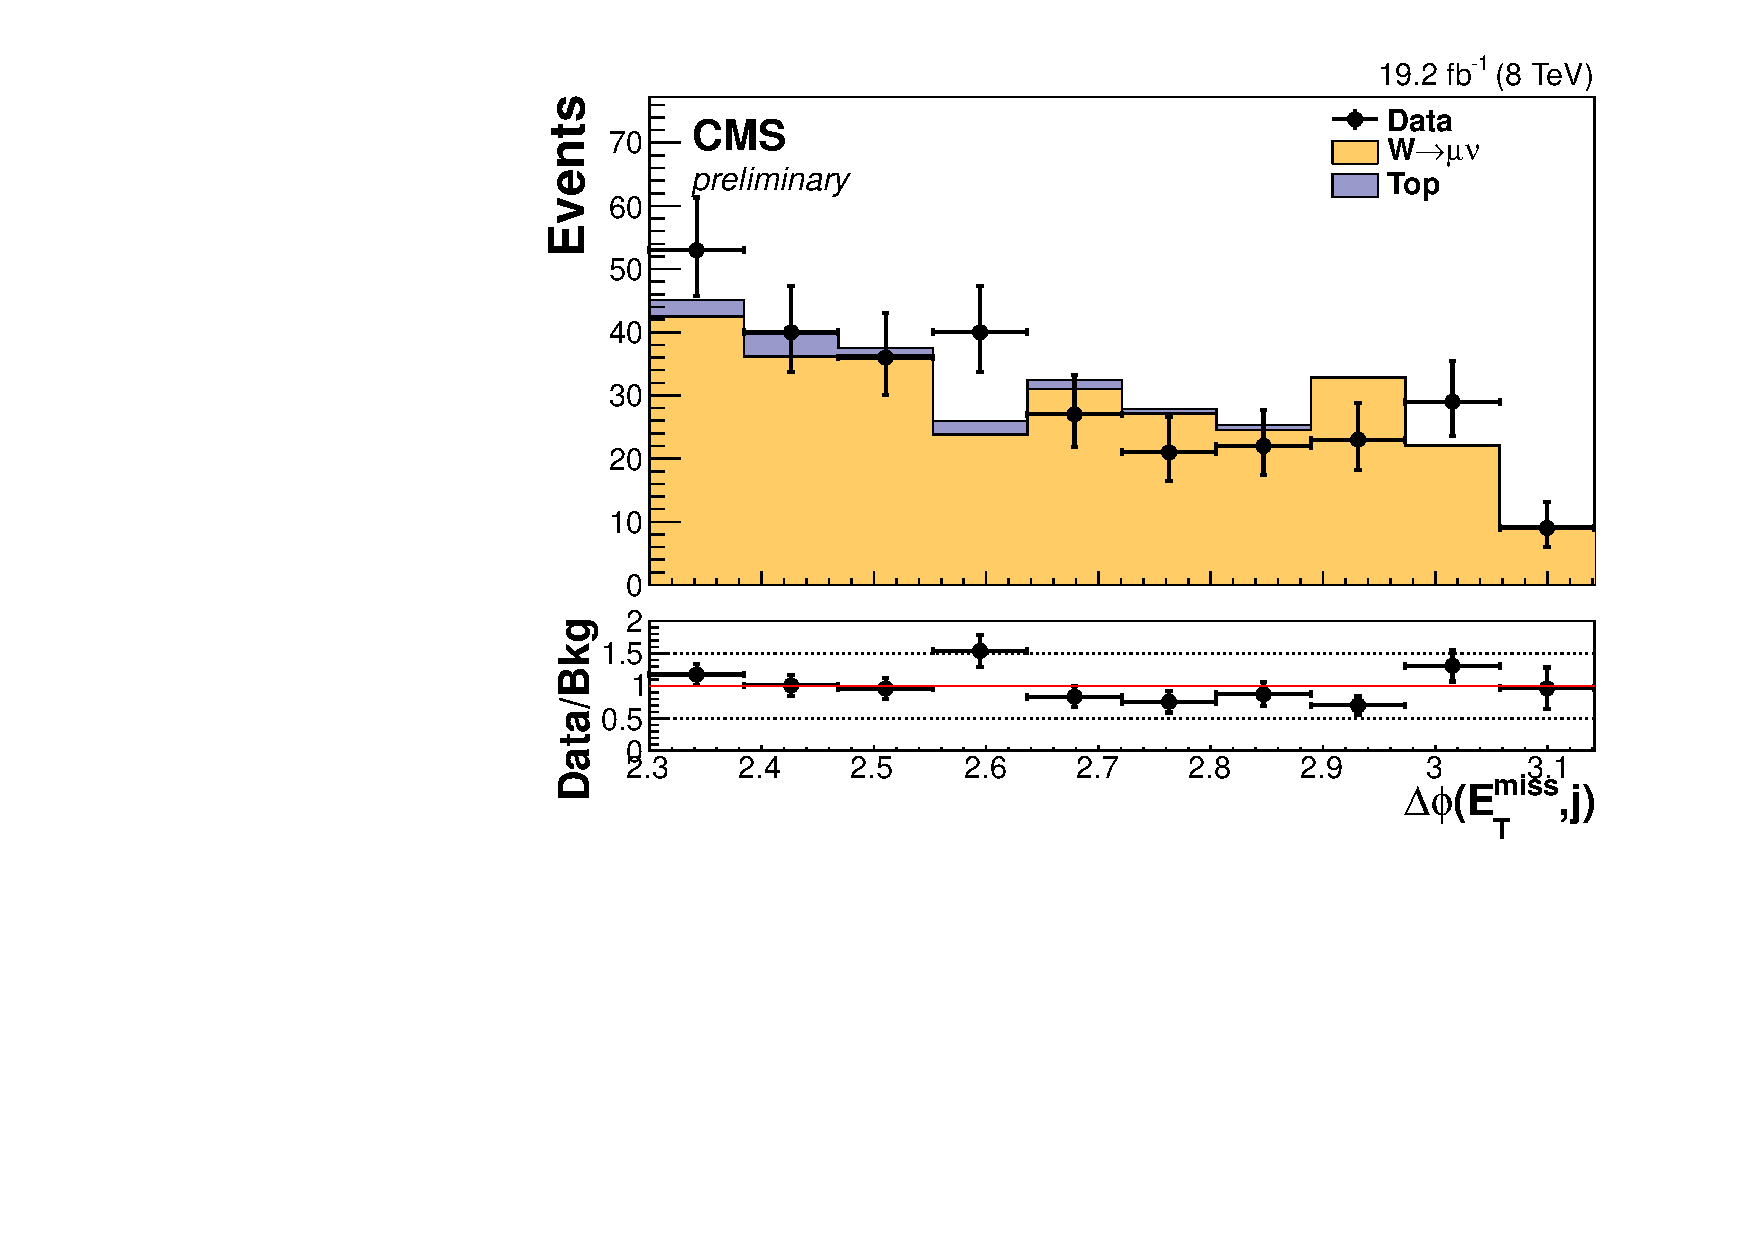
\includegraphics[clip=true,trim=0 0 0 0,width=1.1\textwidth]{TalkPics/IOP2015/output_sigreg/munu_alljetsmetnomu_mindphi.pdf}
      \column{.1\textwidth}
      \hspace{-.5cm}
      \begin{turn}{-90}\scriptsize CMS-PAS-HIG-14-038 \end{turn}
      \end{columns}
      \column{.55\textwidth}
        $Z\rightarrow\nu\nu$ control region
      \begin{columns}
        \column{.9\textwidth}
      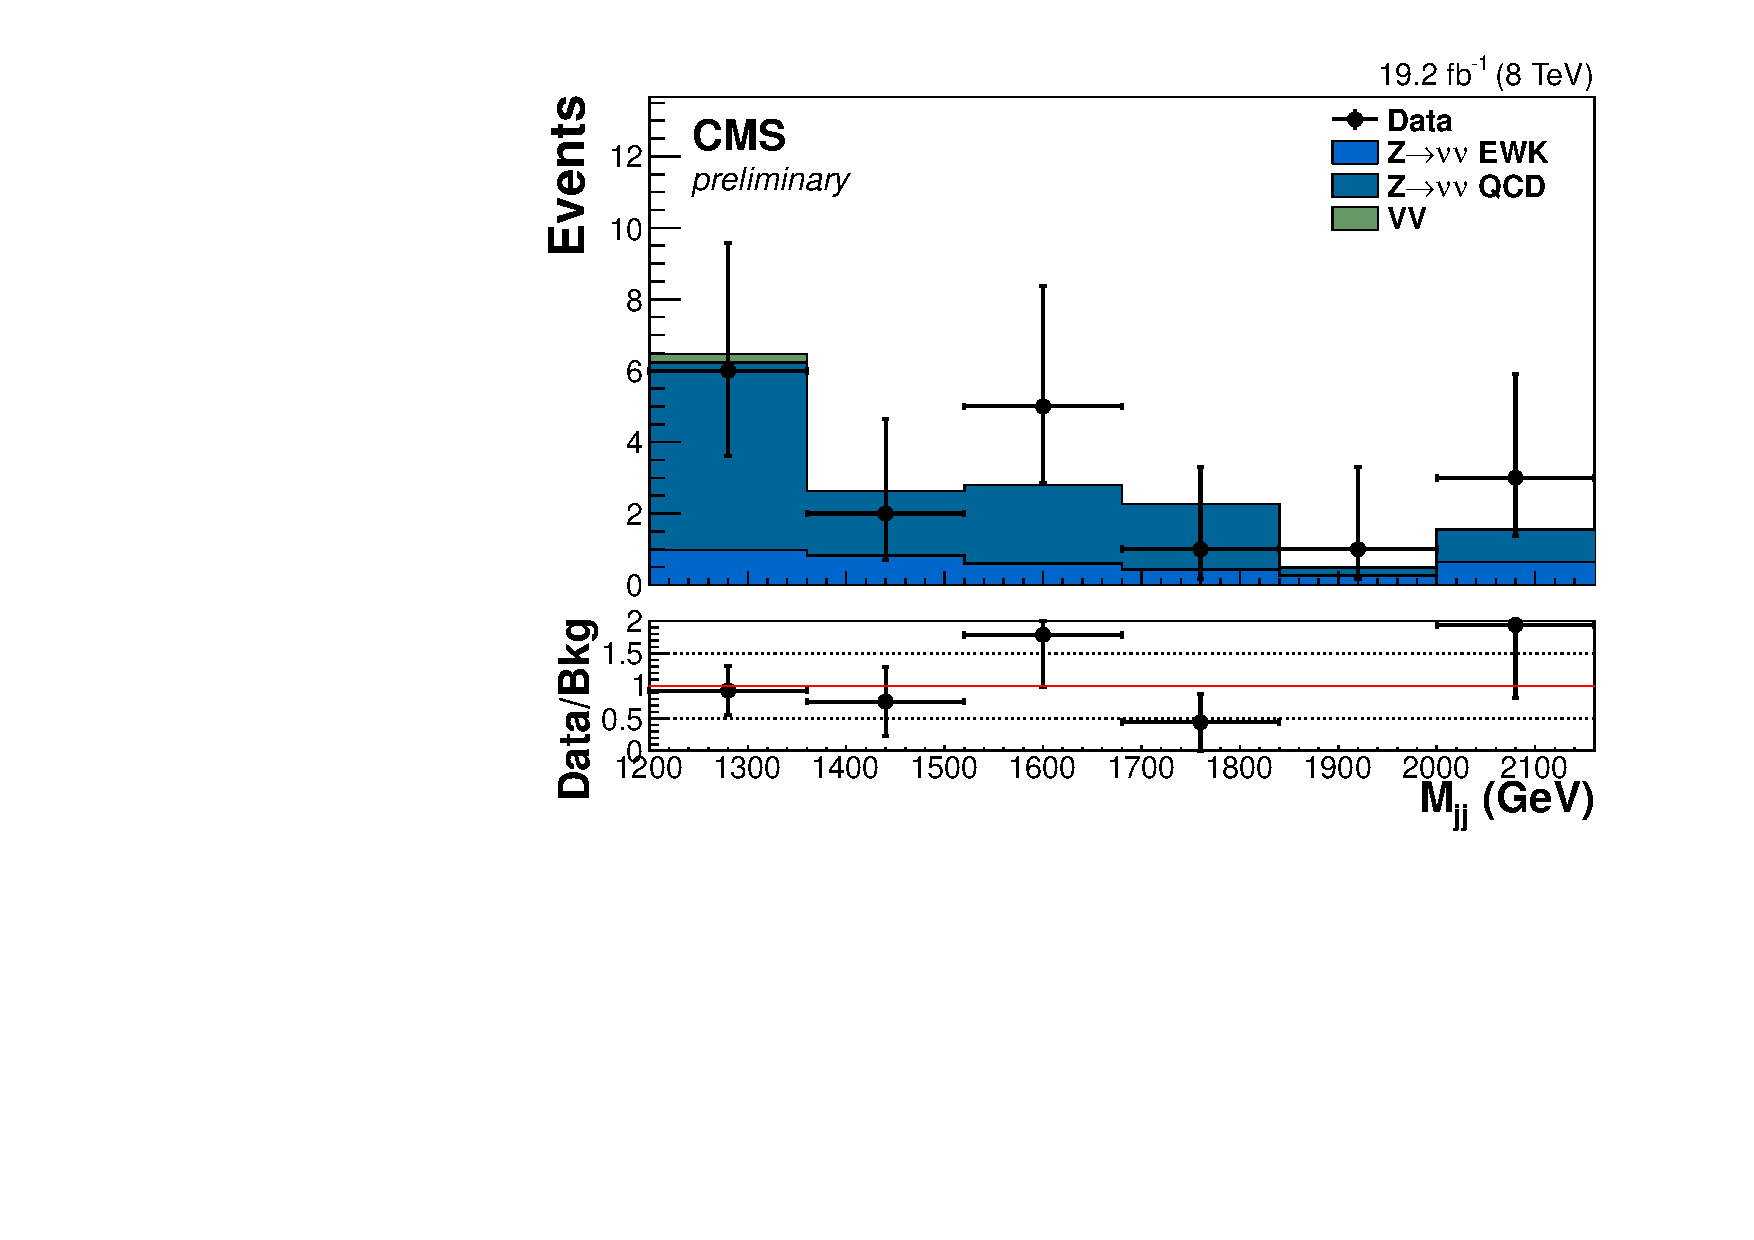
\includegraphics[clip=true,trim=0 0 0 0,width=1.1\textwidth]{TalkPics/IOP2015/output_sigreg/mumu_dijet_M.pdf}
      \column{.1\textwidth}
      \hspace{-.5cm}
      \begin{turn}{-90}\scriptsize CMS-PAS-HIG-14-038 \end{turn}
      \end{columns}
    \end{columns}
  \end{frame}

  \begin{frame}
    \frametitle{What do we see?}
          \scriptsize
          \centering
          \begin{tabular}{lc}
            \hline
            Total background & $439.7\pm 41.0 (stat.) \pm 55.8 (syst.)$ \\ 
            \hline
            VBF H(inv.) assuming B(H$\rightarrow$inv)=100\% &  $273.4 \pm 31.2(syst.)$ \\ 
            ggF H(inv.) assuming B(H$\rightarrow$inv)=100\%& $22.6 \pm 15.6 (syst.)$ \\
            \hline
            Observed data & 508 \\
            \hline
          \end{tabular}
          \normalsize
    \begin{itemize}
    \item No significant excess seen
    \end{itemize}
    \begin{columns}
      \column{.03\textwidth}
      \column{.55\textwidth}
      \begin{columns}
        \column{.9\textwidth}
      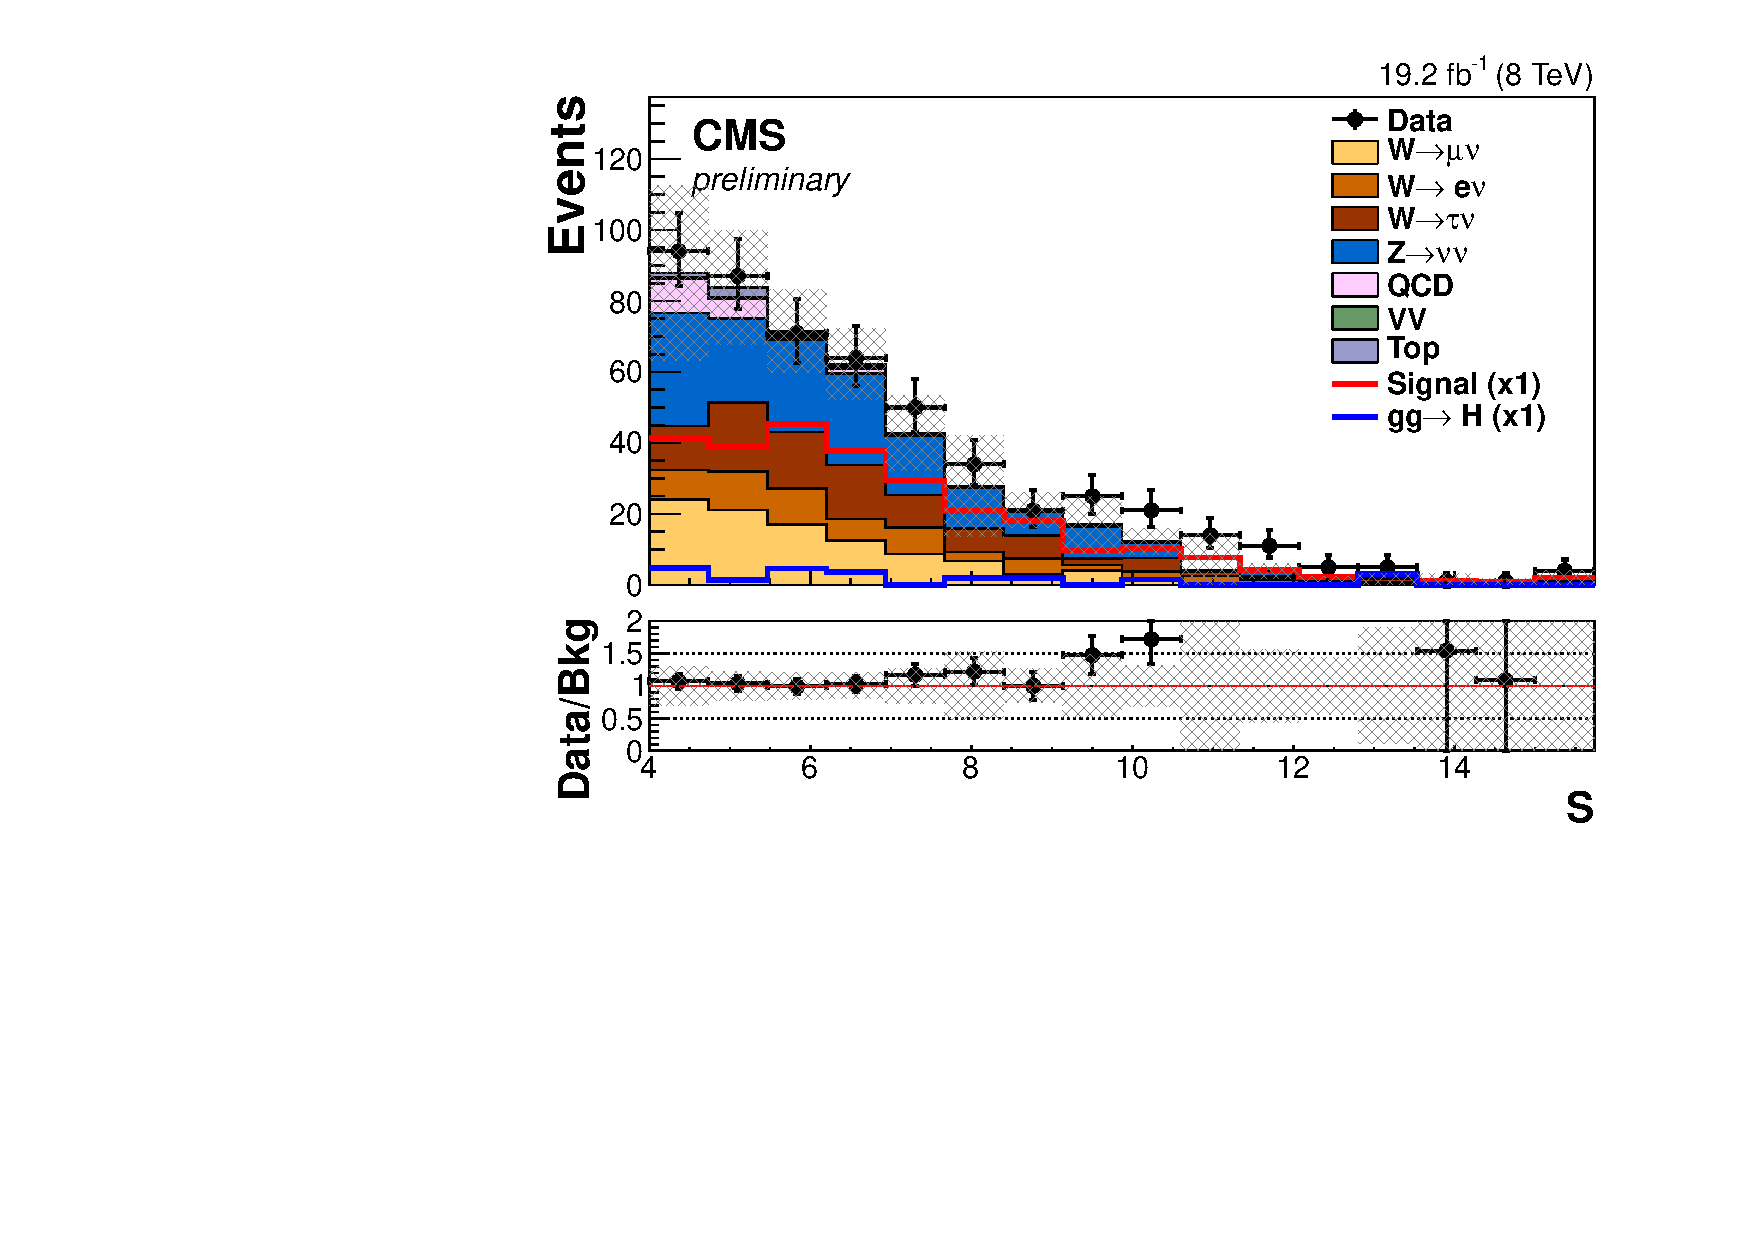
\includegraphics[clip=true,trim=0 0 0 0,width=1.1\textwidth]{TalkPics/IOP2015/output_sigreg/nunu_metnomu_significance.pdf}
      \column{.1\textwidth}
      \hspace{-.5cm}
      \begin{turn}{-90}\scriptsize CMS-PAS-HIG-14-038 \end{turn}
      \end{columns}
      \column{.55\textwidth}
      \begin{columns}
        \column{.9\textwidth}
      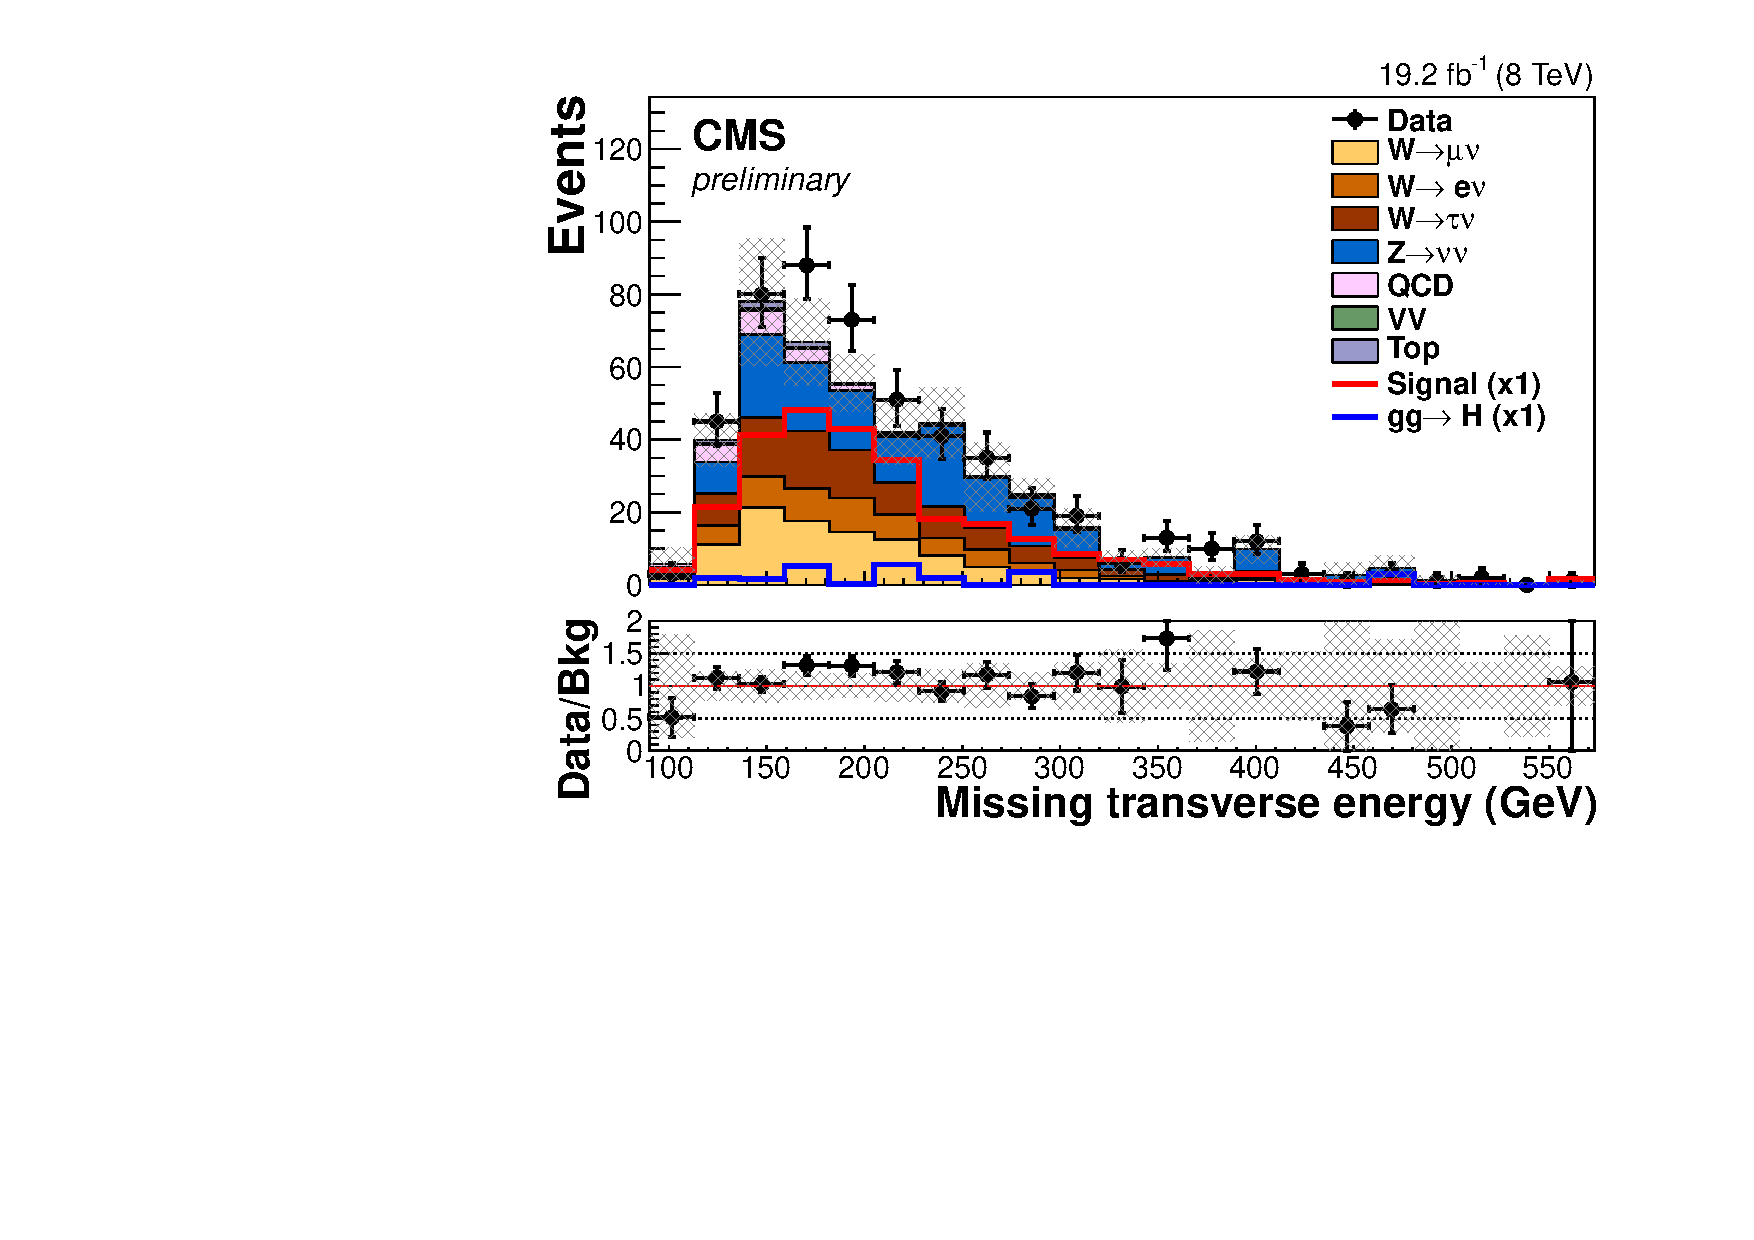
\includegraphics[clip=true,trim=0 0 0 0,width=1.1\textwidth]{TalkPics/IOP2015/output_sigreg/nunu_metnomuons.pdf}
      \column{.1\textwidth}
      \hspace{-.5cm}
      \begin{turn}{-90}\scriptsize CMS-PAS-HIG-14-038 \end{turn}
      \end{columns}
    \end{columns}

  \end{frame}

  \begin{frame}
    \frametitle{What do we see?}
    \begin{columns}
      \column{1.1\textwidth}
      \begin{itemize}
      \item Lack of excess rules out some values of invisible decay rate
        \begin{itemize}
          \color{beamer@icmiddleblue}
        \item VBF alone limits $B(H\rightarrow inv)$ for $m_{H}$=125 GeV to less than 57\%
        \end{itemize}
      \item Combining with other searches the limit is less than 47\%
      \end{itemize}
    \end{columns}
    \begin{columns}
      \column{.03\textwidth}
      \column{.55\textwidth}
      \begin{columns}
        \column{.9\textwidth}
      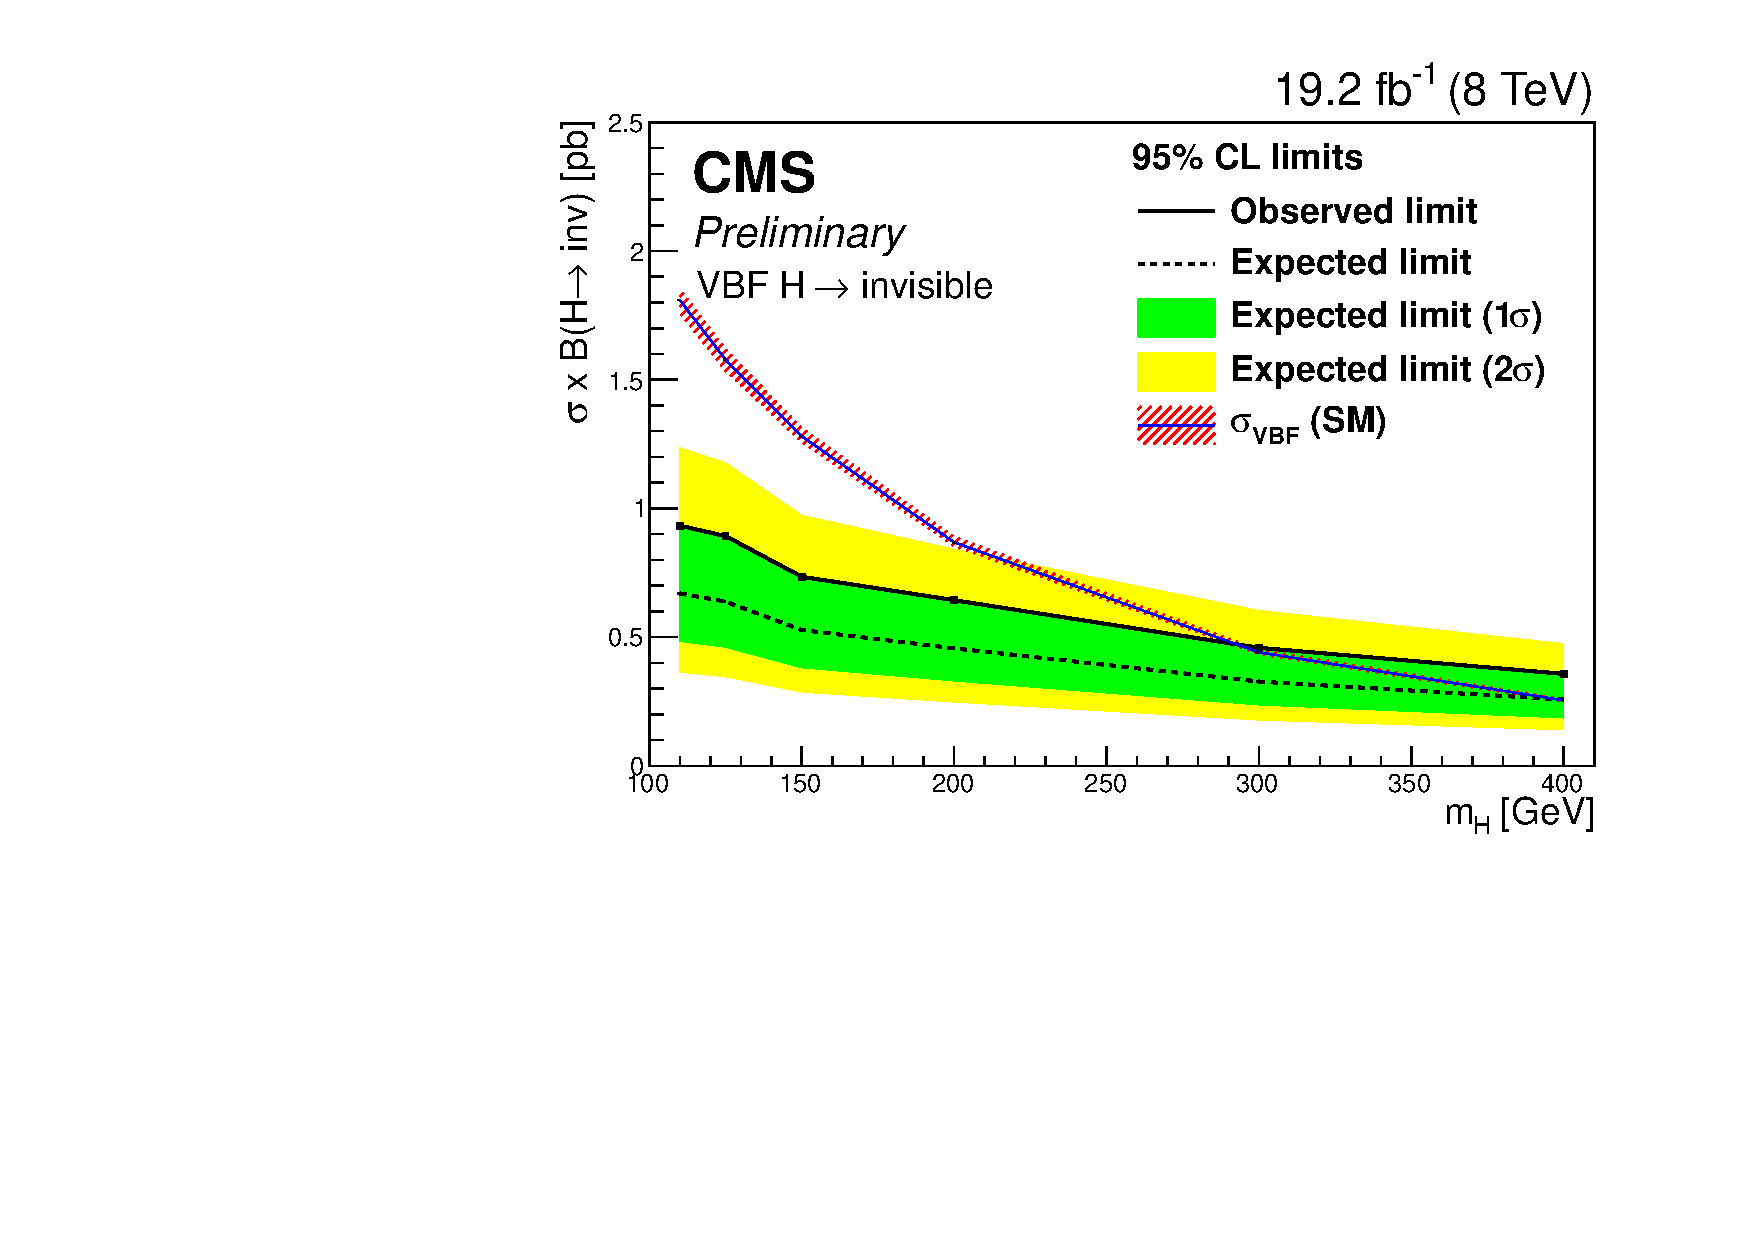
\includegraphics[clip=true,trim=0 0 0 0,width=1.1\textwidth]{TalkPics/IOP2015/vbfxslimit.pdf}
      \column{.1\textwidth}
      \hspace{-.5cm}
      \begin{turn}{-90}\scriptsize CMS-PAS-HIG-14-038 \end{turn}
      \end{columns}
      \column{.55\textwidth}
      \begin{columns}
        \column{.9\textwidth}
      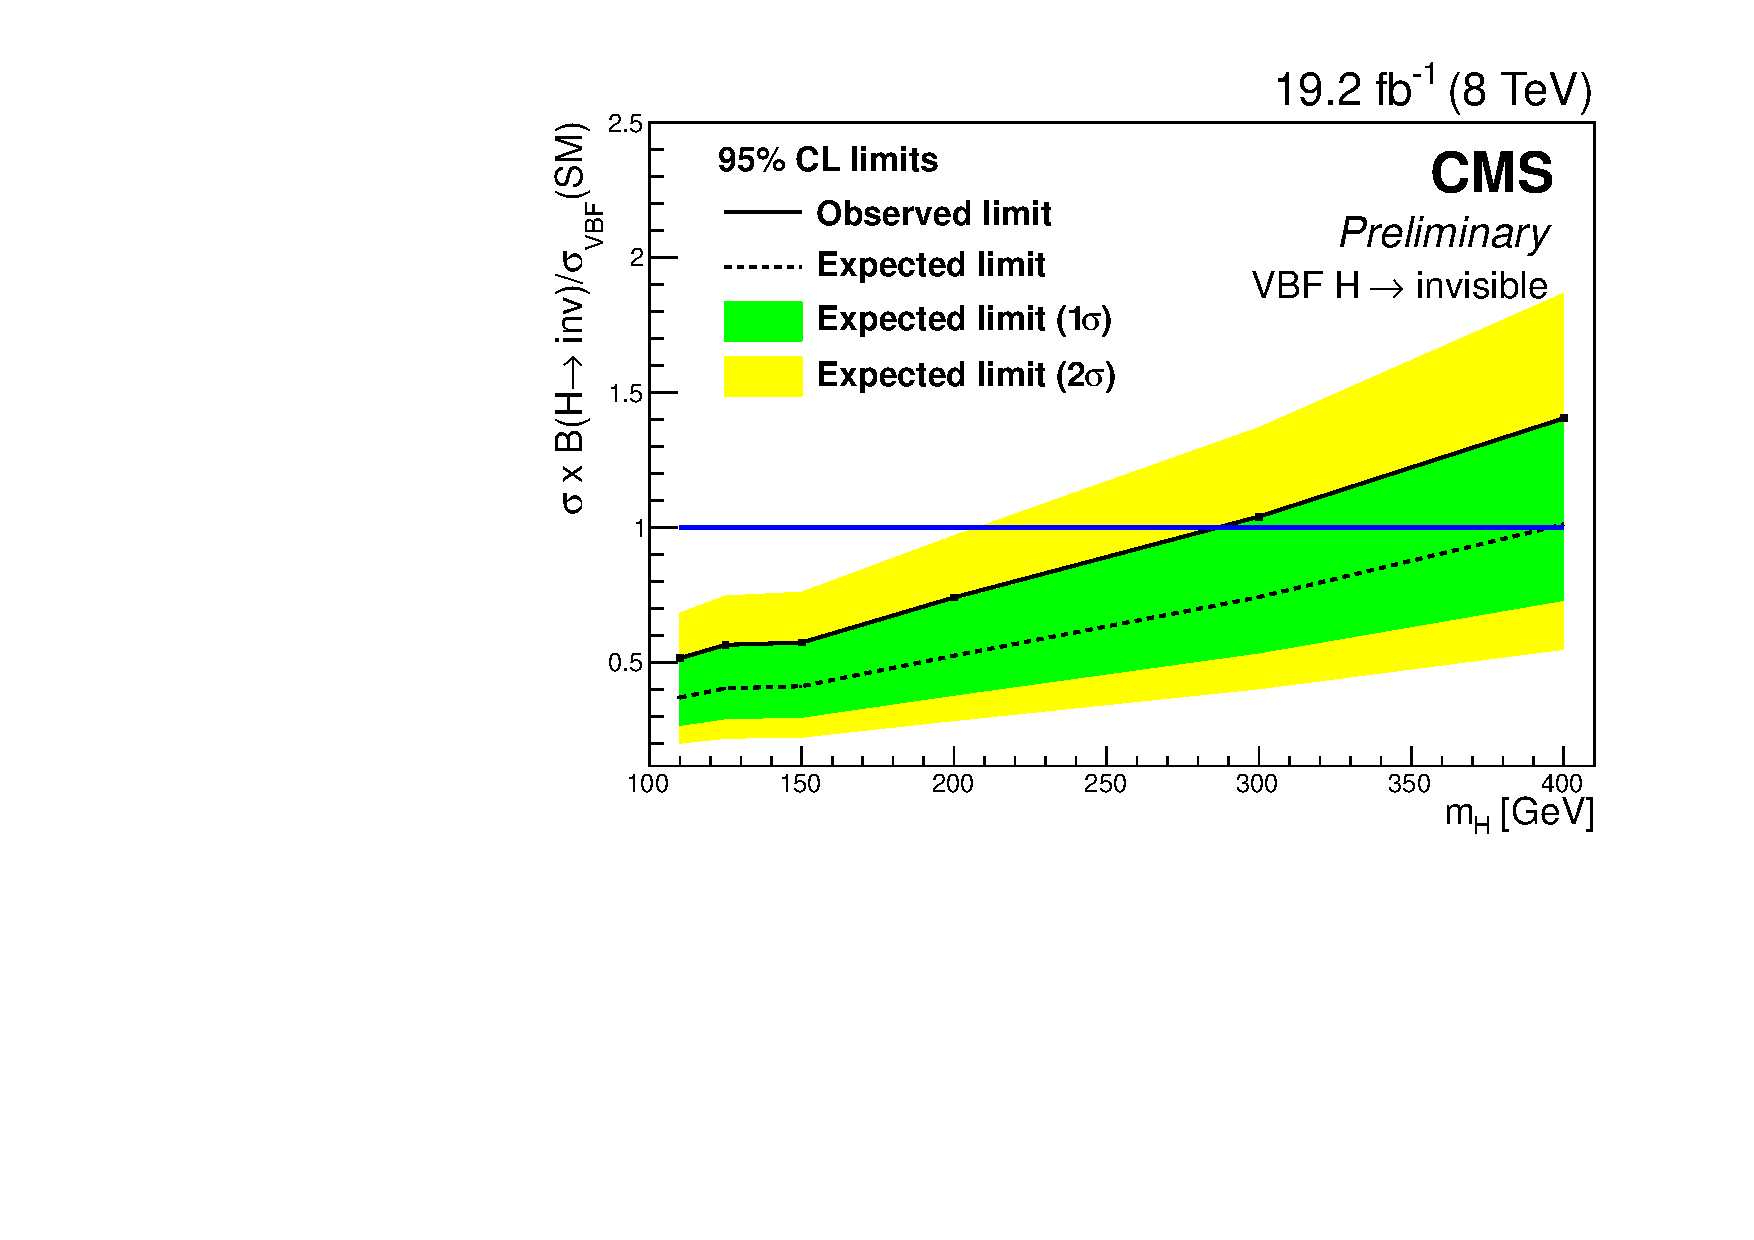
\includegraphics[clip=true,trim=0 0 0 0,width=1.1\textwidth]{TalkPics/IOP2015/vbflimit.pdf}
      \column{.1\textwidth}
      \hspace{-.5cm}
      \begin{turn}{-90}\scriptsize CMS-PAS-HIG-14-038 \end{turn}
      \end{columns}
    \end{columns}
  \end{frame}

  \begin{frame}
    \frametitle{What does this mean for dark matter?}
    %!!Dark matter plot of some sort
  \end{frame}

  \begin{frame}
    \frametitle{Summary}
    \label{lastframe}
    \begin{itemize}
    \item The Higgs discovery is only the beginning
    \item We have already placed tight constraints on Higgs-dark matter interactions
    \item These will become tighter in LHC Run II
    \end{itemize}
    \centering
    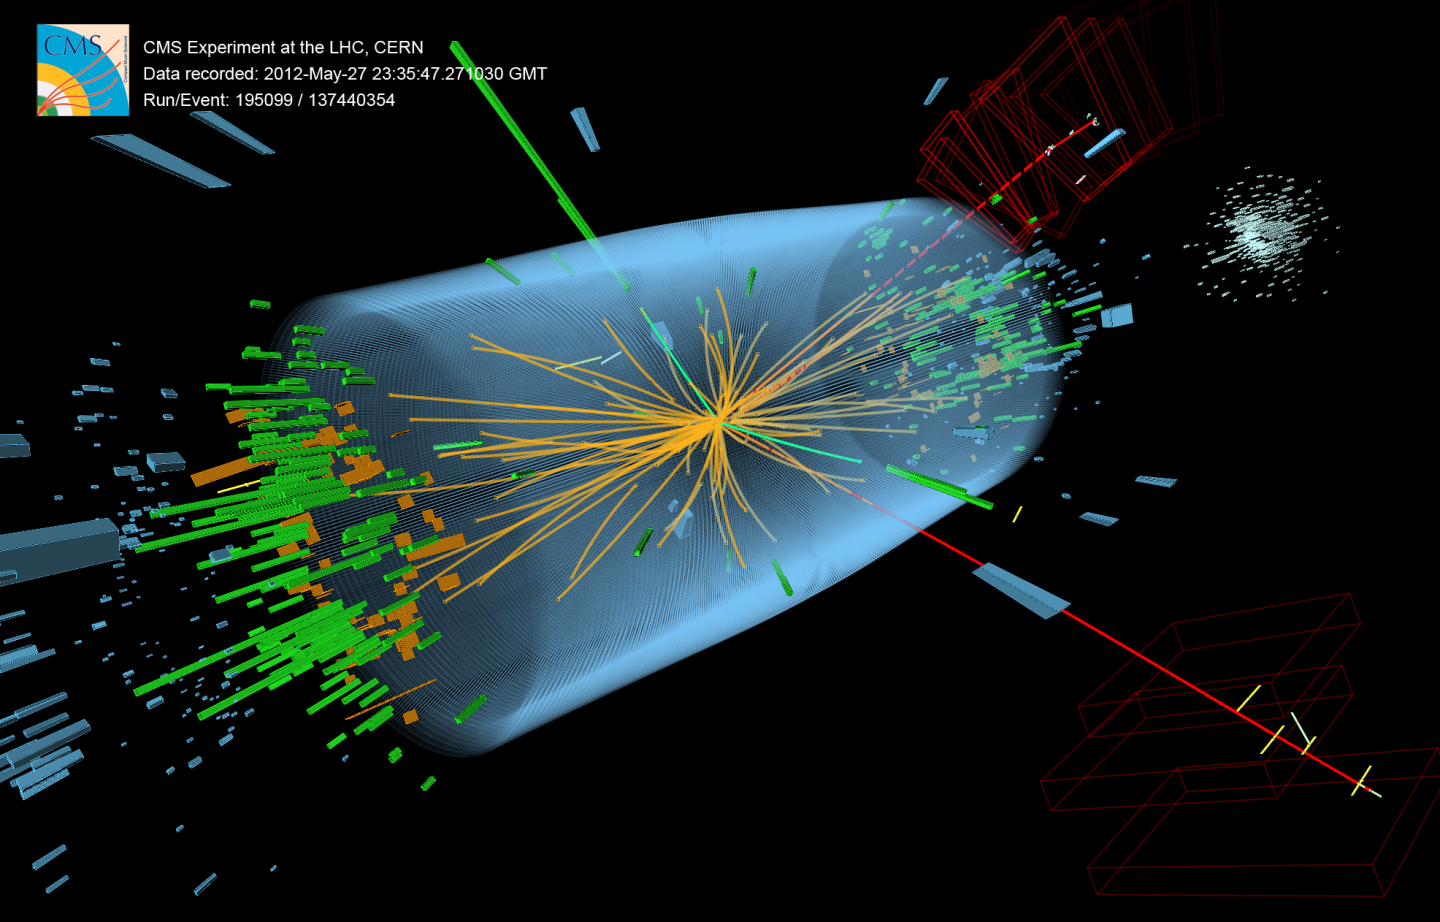
\includegraphics[width=.5\textwidth]{TalkPics/sgs120315/eventdisplay.png}
  \end{frame}
  
  %HIGGS BACKGROUND
  \begin{frame}
    \frametitle{The Higgs Boson}
    \begin{columns}
      \column{.5\textwidth}

      \column{.5\textwidth}

    \end{columns}
  \end{frame}

  \begin{frame}
    \frametitle{What do I do?}
    \centering
    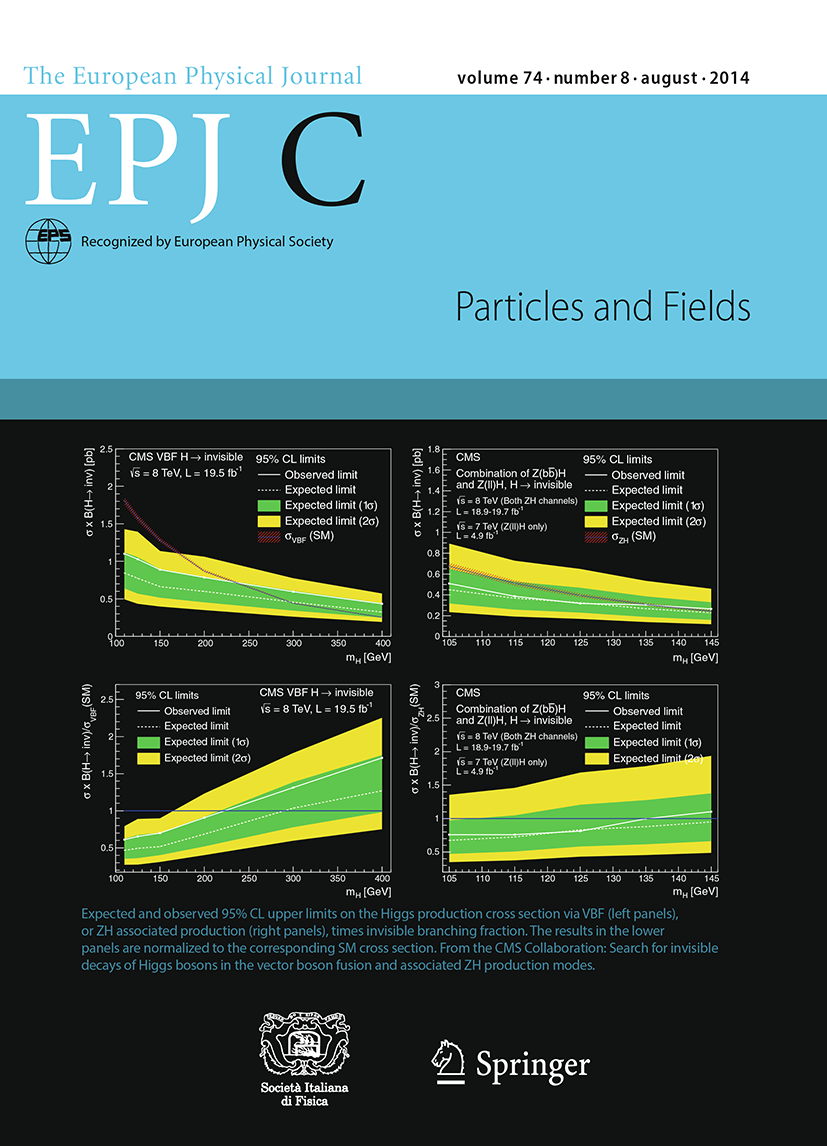
\includegraphics[height=.85\textheight]{TalkPics/EPJCAug2014Cover.png}
  \end{frame}

  \begin{frame}
    \frametitle{Why Higgs to Invisible?}
    \vspace{-.2cm}
    \begin{columns}
      \column{.5\textwidth}
      \begin{block}{\scriptsize Experimental motivation}
        \scriptsize
        \begin{itemize}
        \item Current measurements of the 125 GeV Higgs boson are compatible with Standard Model (SM) expectations
        \item[-] large uncertainties can still accommodate significant beyond the SM (BSM) properties
        \item Additional Higgs bosons with exotic decays are not excluded
        \end{itemize}
      \end{block}
      \column{.45\textwidth}
      \hfill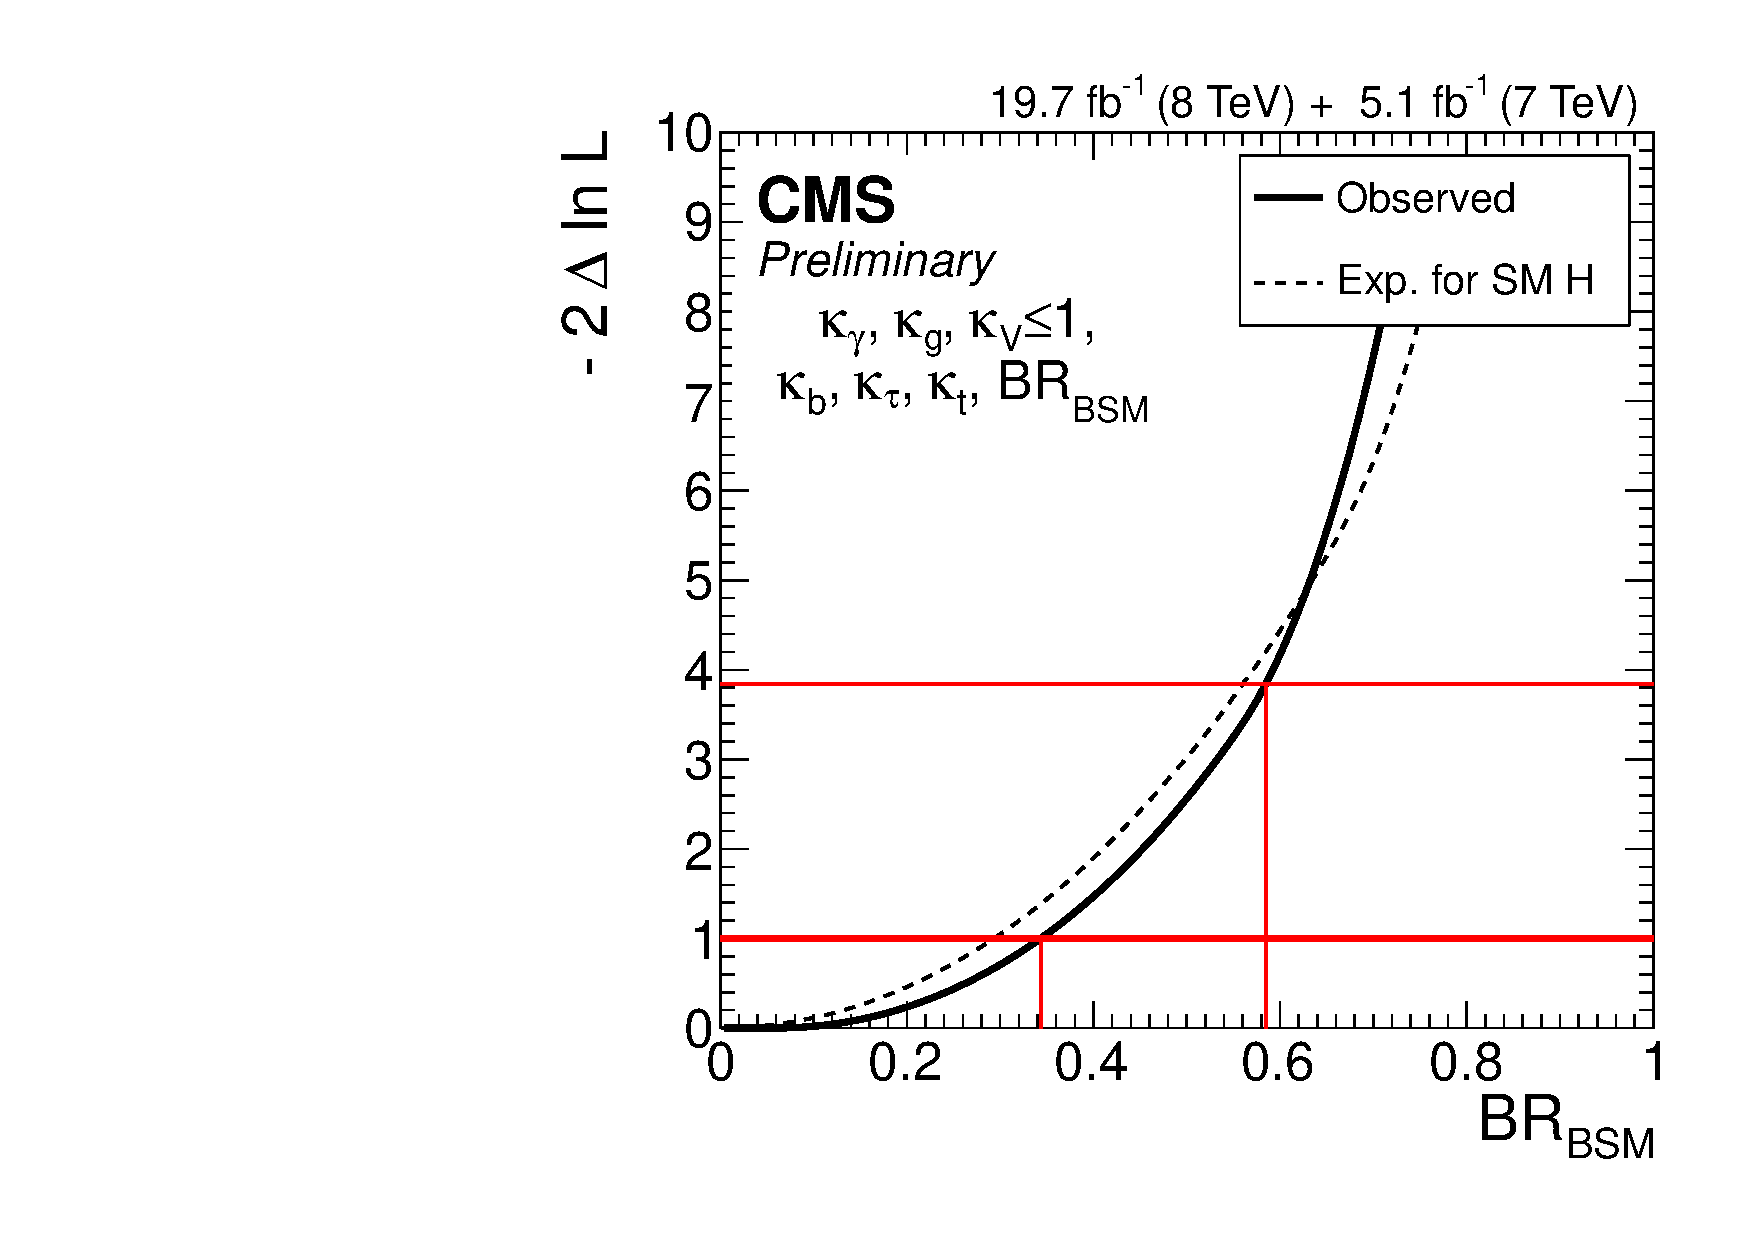
\includegraphics[height=.55\textheight]{TalkPics/panicpics/indirectbrbsm.pdf}
      \column{.05\textwidth}
      \begin{turn}{-90}\scriptsize CMS-PAS-HIG-14-009\end{turn}
    \end{columns}
    \begin{columns}
      \column{1.095\textwidth}
      \begin{block}{\scriptsize Theoretical motivation}
        \scriptsize
        \begin{itemize}
        \item Many BSM theories predict Higgs boson decays to invisible final states:
        \item[-] e.g. SUSY, extra dimensions, fourth-generation neutrinos
        \item These final state particles are often dark matter candidates
        \end{itemize}
      \end{block}
    \end{columns}

  \end{frame}

  %!!SIMPLIFY ALL FROM HERE
  %!!EXPLAIN DATA FLOW AND HOW TO DO AN ANALYSIS

\end{fmffile}
\end{document}

